%
% preamble.tex -- additional packages, loaded by main.tex after wacv.sty and
% before hyperref. (xcolor is loaded by wacv.sty with [dvipsnames]; the `table'
% option is pre-passed in main.tex so \rowcolor works.)
%

% --- figures, math, tables
\usepackage{graphicx}
\usepackage{amsmath,amssymb}
\usepackage{booktabs}
\usepackage{array}
\usepackage{multirow}
\usepackage{enumitem}   % compact list spacing (itemize/enumerate options)
\usepackage{tikz}       % pipeline / flow diagram
\usetikzlibrary{arrows.meta,positioning,backgrounds,fit,shapes.geometric,calc}
\usepackage{pgfplots}   % result charts (scatter / line / bar plots)
\pgfplotsset{compat=1.18}

% --- Fonts: tectonic compiles with XeTeX, whose Unicode (TU) encoding has no
% bold/italic shape for the kit's Type1 Times (ptm) -> \textbf/\textit silently
% render non-bold. TeX Gyre Termes / Heros are Times/Helvetica clones with the
% full set of OpenType shapes, restoring bold and italic.
\usepackage{iftex}
\ifXeTeX
  \usepackage{fontspec}
  \setmainfont{texgyretermes}[
    Extension=.otf, UprightFont=*-regular, BoldFont=*-bold,
    ItalicFont=*-italic, BoldItalicFont=*-bolditalic]
  \setsansfont{texgyreheros}[
    Extension=.otf, UprightFont=*-regular, BoldFont=*-bold,
    ItalicFont=*-italic, BoldItalicFont=*-bolditalic]
\fi

% --- Teaser pipeline (Figure 1), emitted at the top of page 1 ---------------
% wacv's \maketitle wraps \@maketitle in \twocolumn[...]; the page-1 top region
% is thus title matter and a figure* float declared in the body defers to page 2.
% We inject the full-width pipeline into that top matter so it lands at the very
% top of page 1, above the abstract, numbered Figure~1. Its counter step and
% \label{fig:pipeline} are done in the body (top of sec/1_intro) for pass-stable
% numbering; the caption number is therefore hardcoded "Figure~1.".
\newcommand{\pipelineteaser}{%
  \vspace{0pt}\par\noindent
  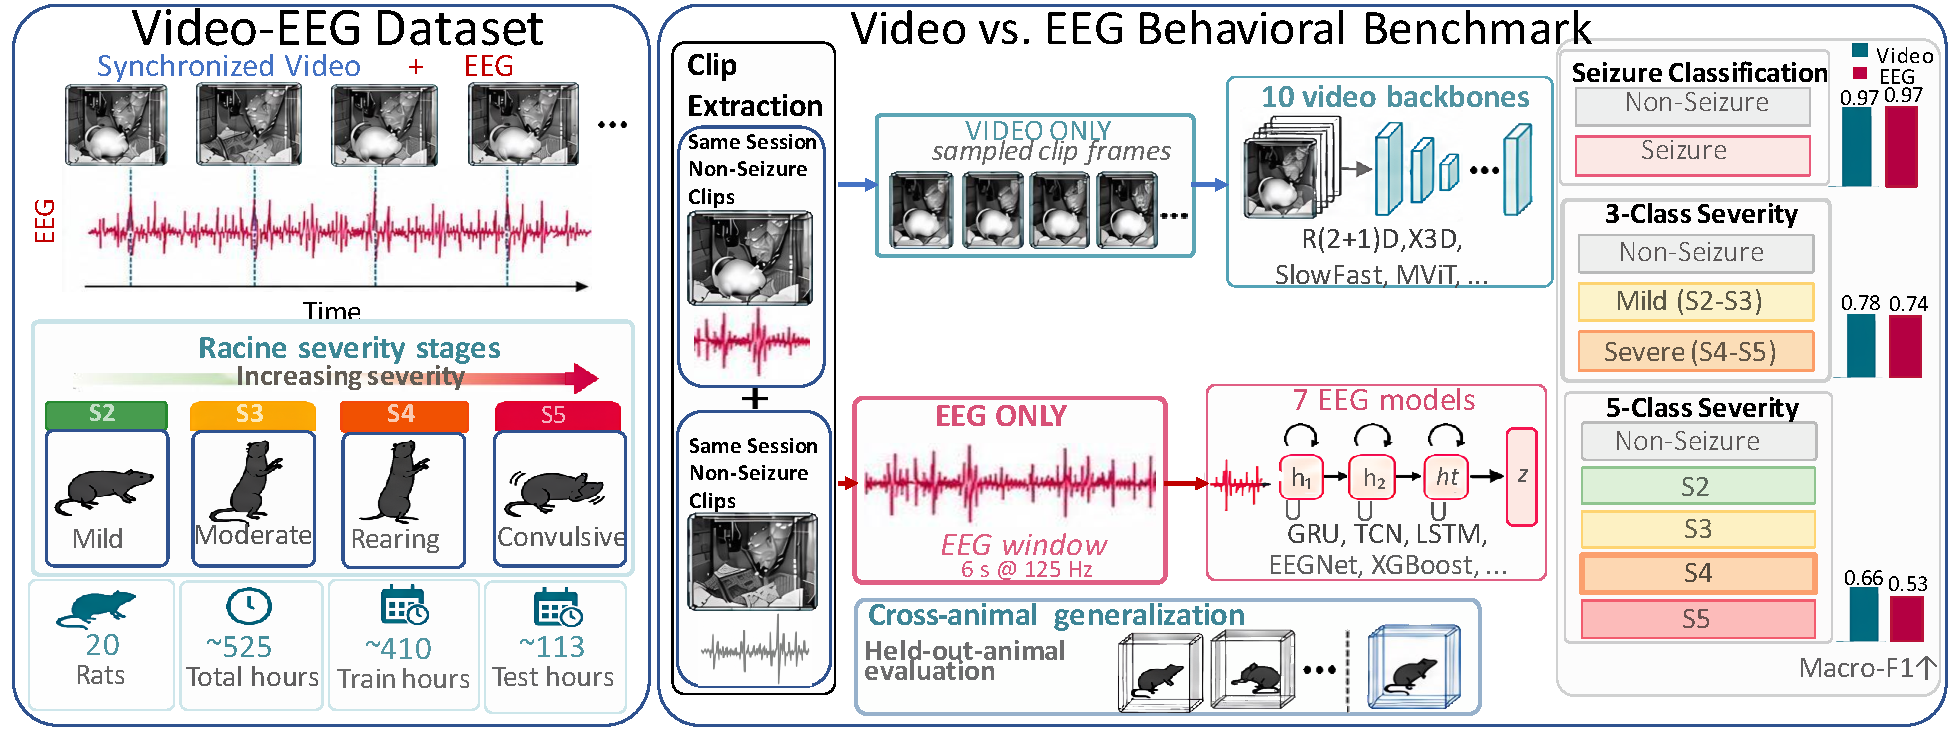
\includegraphics[width=\textwidth]{fig/fig_pipeline.pdf}%
  \par\vspace{2pt}
  {\small Figure~1.\hspace{0.5em}Overview of the study. \emph{Left:} the cohort---
  synchronized video and EEG from 20 rats (corpus scale in
  App.~\ref{sec:dataextra:cohort}, Table~\ref{tab:corpusscale}), each clip graded on the
  Racine scale from Stage\,2 (mild) to Stage\,5 (convulsive). \emph{Right:} the
  benchmark. Expert-annotated seizure clips and same-session non-seizure clips feed
  two independent, unfused lanes---ten video backbones and seven EEG models---%
  compared head-to-head at 2-, 3- and 5-class granularity and under
  held-out-animal evaluation. Bars report macro-F1: the two modalities are level
  at detection and separate as the task becomes explicitly behavioral.\par}%
  \vspace{3pt}%
}
% Append the teaser pipeline to the (two-column-spanning) title top matter.
\makeatletter
\g@addto@macro\@maketitle{\pipelineteaser}
\makeatother

% --- Key-takeaway callout -------------------------------------------------
% A tinted box closing each results subsection with its one-line conclusion.
% Colour matches wacvblue (main.tex), redefined here since preamble is input first.
\usepackage[most]{tcolorbox}
\definecolor{takeawayaccent}{rgb}{0.21,0.49,0.74}
\newtcolorbox{takeaway}{
  enhanced,
  colback=takeawayaccent!6, colframe=takeawayaccent!55,
  boxrule=0.5pt, arc=2pt,
  left=5pt, right=5pt, top=3.5pt, bottom=3.5pt,
  before skip=6pt, after skip=6pt,
  fontupper=\small,
}
\newcommand{\takeawaylabel}{\textbf{\textcolor{takeawayaccent!80!black}{Key takeaway.}}\ }

% --- inline annotations (from the kit)
\newcommand{\red}[1]{{\color{red}#1}}
\newcommand{\todo}[1]{{\color{red}#1}}
\newcommand{\TODO}[1]{\textbf{\color{red}[TODO: #1]}}
% --- disable by uncommenting
% \renewcommand{\TODO}[1]{}
% \renewcommand{\todo}[1]{#1}
